\section{GPIO}
\begin{figure}[h!]
    \centering
    \includegraphics[width=0.7\textwidth]{../organization/GPIO.pdf}
    \caption{Blockschaltbild GPIO}
    \label{fig:block}
\end{figure}
\noindent Mit der GPIO sind die Schalter, Taster und LED ans Bussystem der MCU 
angeschlossen. Die Taster und Schalter werden Synchronisiert um Metastabilität 
zu vermeiden. Der Floppy Controller wird ebenfalls via GPIO Modul ans 
Bussystem angebunden. 

\subsection{Memory Map}
\begin{table}[h!]
    \centering
    \begin{zebratabular}{lll}
        \rowcolor{gray}
        Addresse  & Register          & R/W   \\
        0x80      & Switch            & R     \\
        0x81      & LED               & R/W   \\
    \end{zebratabular}
    \caption{Memory Map}
    \label{tab:mem_map}
\end{table}
